\begin{frame}
\frametitle{Directed graphs}
\begin{itemize}

\pause
\item \inote{(AKA Digraph)} Order matters

\pause
\item Undirected edge is \alert{set of one or two} vertices (eg. $\{A, B\}$)

\pause
\inote{In sets, order doesn't matter, so $\{A, B\}$ could have been $\{B, A\}$. This won't do for directed graphs}

\pause
\item Directed edge is \alert{ordered pair} of vertices (eg. $(A, B)$)

\pause
\inote{How would you encode a self-loop, since you have to have an ordered \textbf{pair}?}

\pause
\item $G = (V, E)$, just like old times
\end{itemize}
\end{frame}

\begin{frame}
\frametitle{Directed graph example}

\pause
\begin{example}
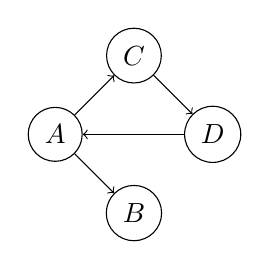
\begin{tikzpicture}
\node (A) at (0, 2) [circle,draw] {$A$};
\node (B) at (1, 1) [circle,draw] {$B$};
\node (C) at (1, 3) [circle,draw] {$C$};
\node (D) at (2, 2) [circle,draw] {$D$};

\draw[->] (A) to (B);
\draw[->] (A) to (C);
\draw[->] (C) to (D);
\draw[->] (D) to (A);
\end{tikzpicture}
\end{example}

\begin{itemize}
\pause
\item Adjacent to $A$:
\pause $B, C$ \inote{Since $A$ is connected to $B$ and $C$, not $D$}

\pause
\item  $\deg^- A = $
\pause 1 \inote{in-degree, arrows pointing into $A$}

\pause
\item $\deg^+ A = $
\pause 2 \inote{out-degree, arrows pointing out of $A$}

\pause
\item See a cycle?
\pause $[D, A, C, D]$ \inote{Path that starts where it stops. Paths can't go against the arrows}
\end{itemize}
\end{frame}

\begin{frame}
\frametitle{Binary relations}
\begin{itemize}
\pause
\item Arbitrary binary relation $R = \{(1, 2), (1, 3), (3, 4), (4, 1)\}$

\pause
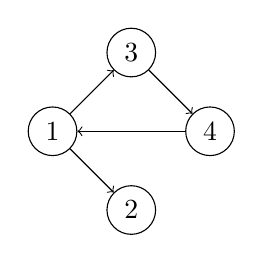
\begin{tikzpicture}
\node (1) at (0, 2) [circle,draw] {$1$};
\node (2) at (1, 1) [circle,draw] {$2$};
\node (3) at (1, 3) [circle,draw] {$3$};
\node (4) at (2, 2) [circle,draw] {$4$};

\draw[->] (1) to (2);
\draw[->] (1) to (3);
\draw[->] (3) to (4);
\draw[->] (4) to (1);
\end{tikzpicture}

\pause
\item Partially ordered set (poset)

\pause
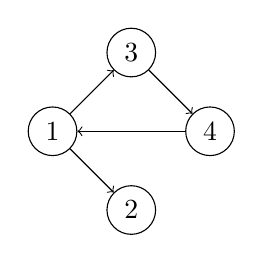
\begin{tikzpicture}
\node (1) at (0, 2) [circle,draw] {$1$};
\node (2) at (1, 1) [circle,draw] {$2$};
\node (3) at (1, 3) [circle,draw] {$3$};
\node (4) at (2, 2) [circle,draw] {$4$};

\draw[->] (1) to (2);
\draw[->] (1) to (3);
\draw[->] (3) to (4);
\draw[->] (4) to (1);
\end{tikzpicture}
\end{itemize}
\end{frame}


%%% Local Variables:
%%% mode: latex
%%% TeX-master: "graphs"
%%% End:
